\item \points{7b}

In this question, we'll train the agent with DeepMind's architecture on the Atari \texttt{Pong} environment. Run the following command to start the training process:
\begin{lstlisting}
$ python run.py --config_filename=q7_dqn
\end{lstlisting}
To speed up training, we have trained the model for 5 million steps (these pretrained weights will be automatically loaded once you run the above command). You are responsible for training it to completion, which should take \textbf{8 hours}. You should get a score of around 12-15 after 4 million total time steps.  As stated previously, the DeepMind paper claims average human performance is $ -3 $. Once your model has fully trained download the following file to your local machine ~src/submission/model.weights~ and include these weights with your code submission to Gradescope. 

\textit{Note: the weights file needs to be in the submission folder for the autograder to read them when you run the grader on your local machine.}


As the training time is roughly 8 hours, you may want to check after a few epochs that your network is making progress.  The following are some training tips:

\begin{itemize}
\item If you terminate your terminal session, any training processes which are running within this session will terminate.  In order to avoid this, you can start a session with Tmux which will persist even if you lose your connection to the vm. See the \href{https://github.com/scpd-proed/XCS234-Handouts/blob/main/Azure/Azure%20Guide.pdf}{Azure guide} for further details).
\item The evaluation score printed on terminal should start at -21 and increase.
\item The max of the q values should also be increasing.
\item The standard deviation of q shouldn't be too small. Otherwise it means that all states have similar q values.
\item Please find our Tensorboard graphs from one training session below.
\end{itemize}

\begin{figure}[H]
\centering
  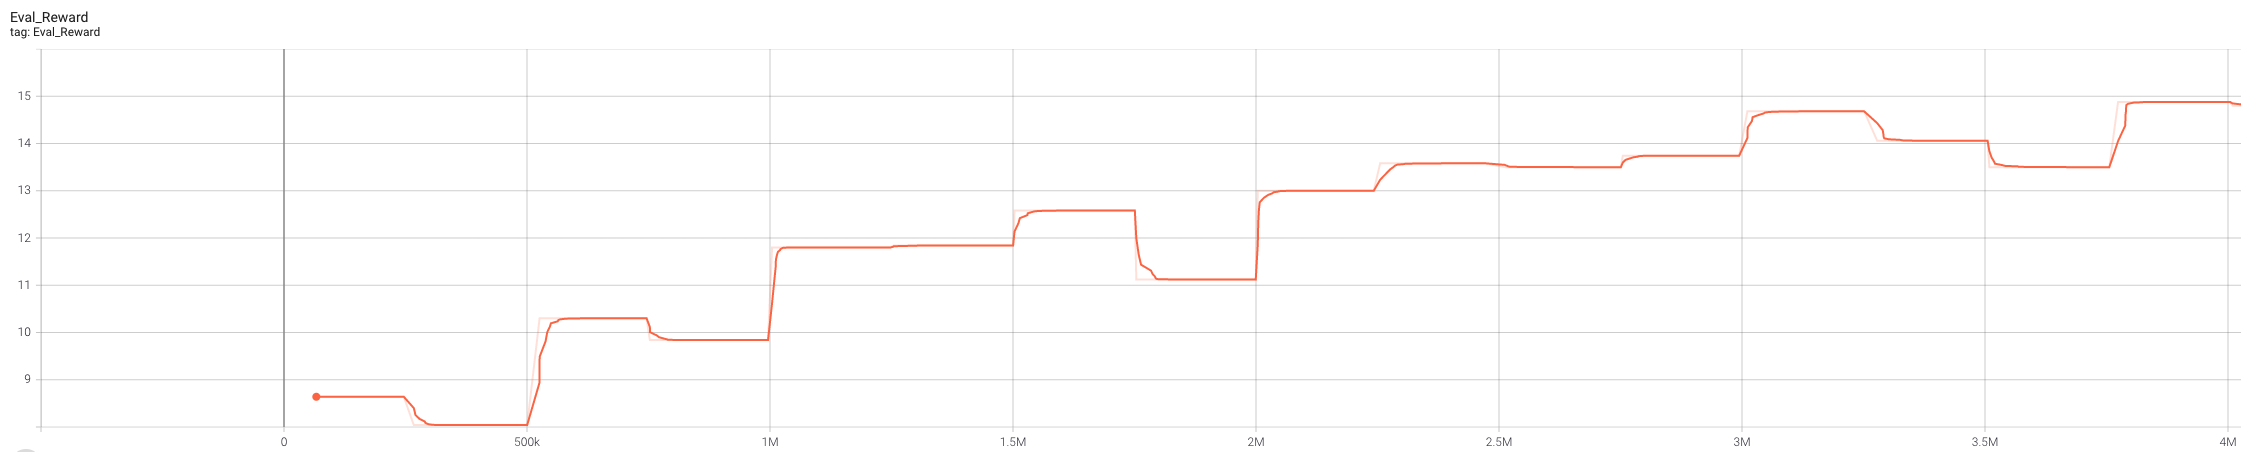
\includegraphics[width=.4\linewidth]{images/Eval_R.png}
  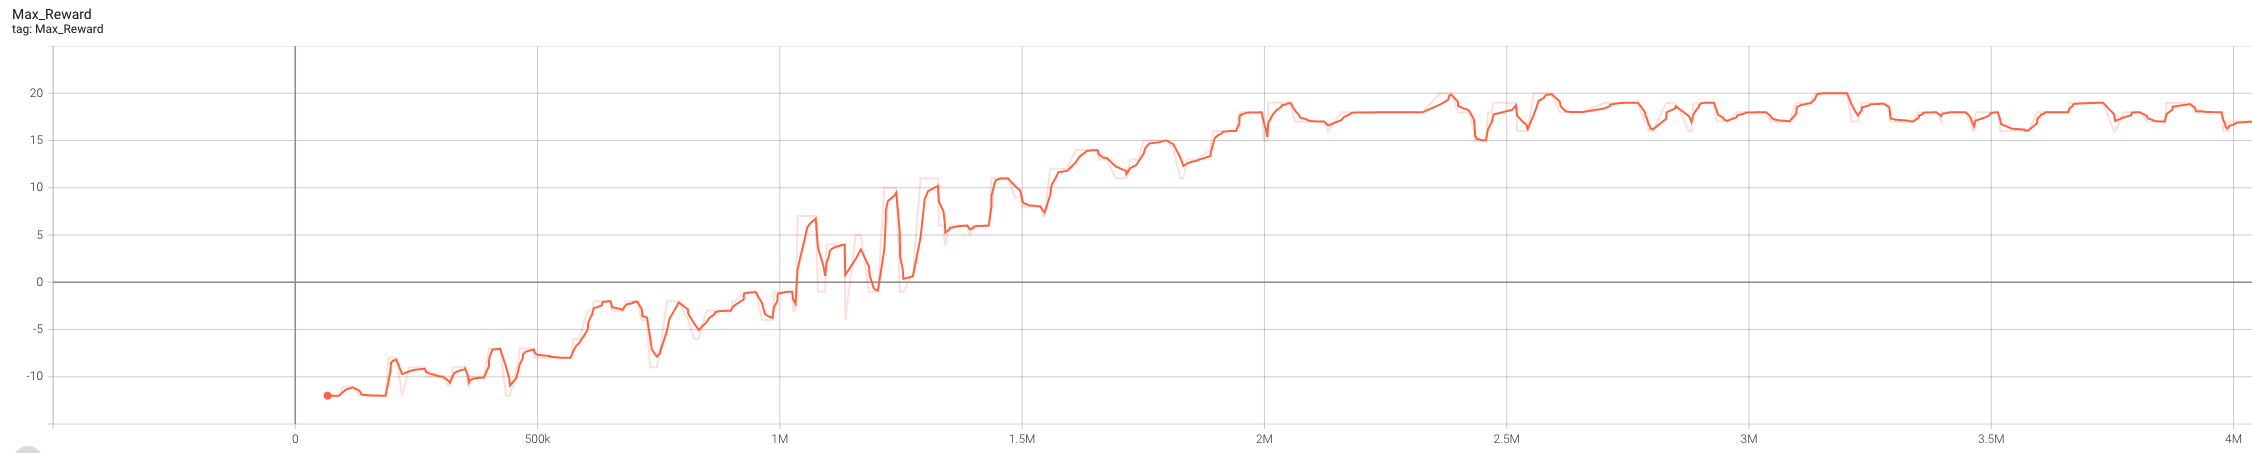
\includegraphics[width=.4\linewidth]{images/Max_R.png}
  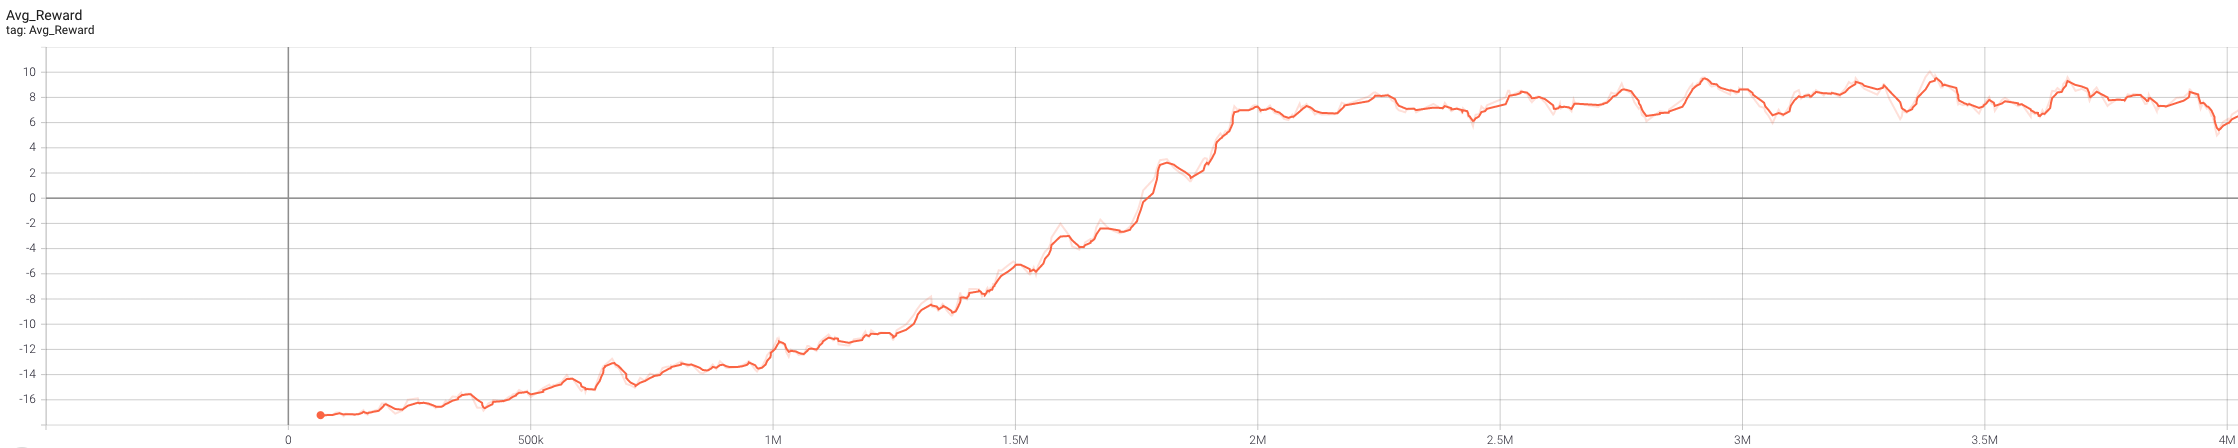
\includegraphics[width=.4\linewidth]{images/Avg_R.png}
  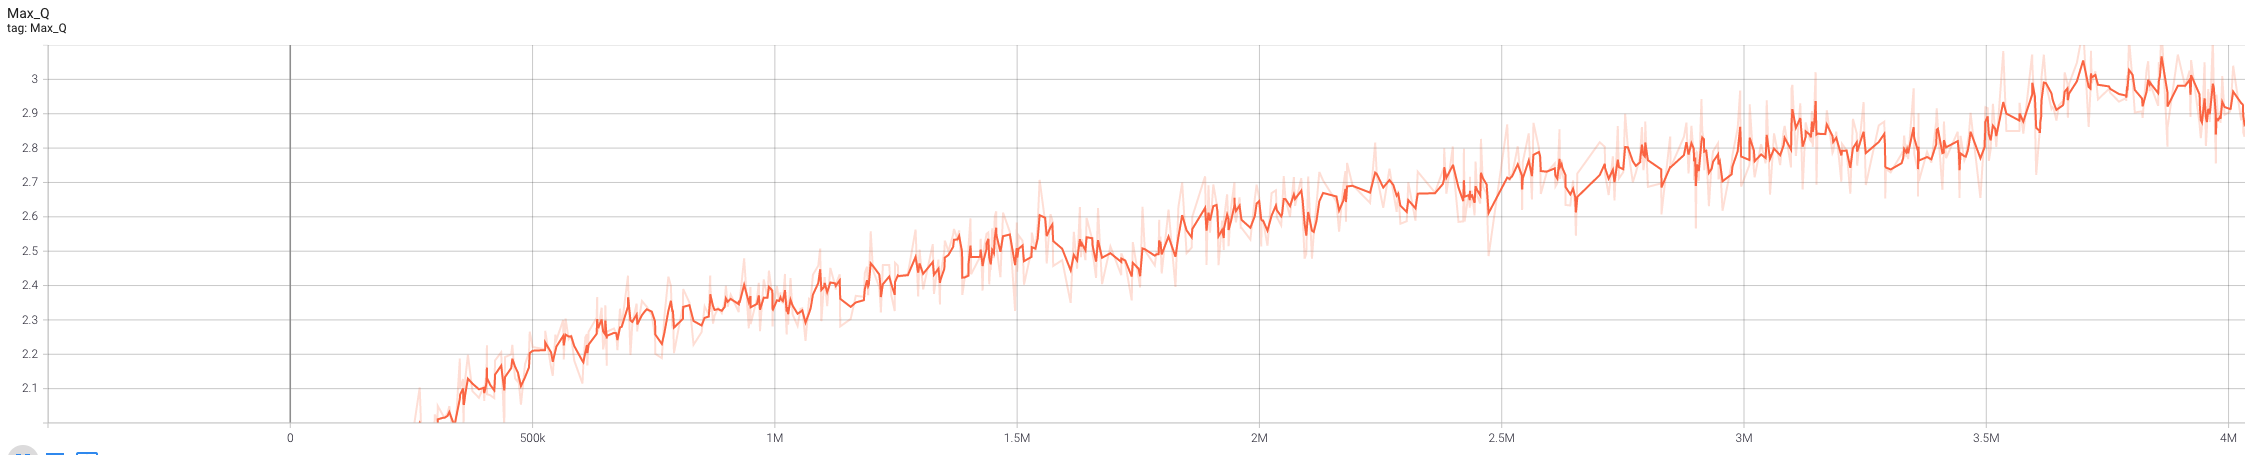
\includegraphics[width=.4\linewidth]{images/Max_Q.png}
\end{figure}